\documentclass[a4paper,12pt,oneside]{article}
\usepackage{amsmath}
\usepackage{mathtools}
% \usepackage{caption}
\usepackage[labelformat=empty]{caption}
\usepackage{mathptmx}
\usepackage{fixltx2e}
\usepackage{graphicx}
\usepackage[margin=1.0in]{geometry}
\usepackage{float}
\let\counterwithout\relax
\let\counterwithin\relax
\usepackage{setspace}
\usepackage{chngcntr}
\usepackage{fancyhdr}
\usepackage{etoolbox}
\patchcmd{\thebibliography}{\section*{\refname}}{}{}{}


\pagestyle{fancy}
\fancyhf{}
\rfoot{\thepage}
%\renewcommand{\headrulewidth}{0.0pt}
%\renewcommand{\footrulewidth}{0.0pt}


\begin{document}
\thispagestyle{empty}
%\pagenumbering{gobble}
\begin{center}

\large{\textbf{{A Smart Home Energy Management System
Using IoT and Big Data Analytics Approach}}}
\setlength{\baselineskip}{1.5\baselineskip}
\\
\vspace{5mm}
\textbf{SEMINAR REPORT}

Submitted in the partial fulfilment of the award of the degree
of
\\
\textbf{Bachelor of Technology}
\\
in
\\
\textbf{Computer Science \& Engineering}
\\
of
\\
\textbf{APJ Abdul Kalam Technological University}
\\
by
\\
\textbf{S HEMANTH}
\\
\vspace{5mm}
\begin{figure}[H]
\centering

\includegraphics[scale=0.5]{ceclogo.png}
\end{figure}
\textbf{November 2019}
\vspace{8mm}
\\
Department of Computer Engineering
\\
College of Engineering, Chengannur, Kerala -689121
\\
Phone: (0479) 2454125, 2451424; Fax: (0479) 2451424
\\
\end{center}

\newpage
\thispagestyle{empty}
\begin{center}
\setlength{\baselineskip}{1.5\baselineskip}
{\large\textbf{COLLEGE OF ENGINEERING, CHENGANNUR}}
\\
{\large\textbf{KERALA}}
\\
\begin{figure}[H]
\centering

\includegraphics[scale=0.5]{ceclogo.png}
\end{figure}
\setlength{\baselineskip}{1.5\baselineskip}
\textbf{Department of Computer Engineering}
\\
\textbf{CERTIFICATE}
\\
This is to certify that the seminar entitled
\\
\textbf{A Smart Home Energy Management System
Using IoT and Big Data Analytics Approach}
\\
Submitted by
\\
\textbf{S HEMANTH}
\\
is a bonafide record of the work done by him.
\end{center}
\vspace{30ex}
%\textbf{Mrs.Sheeba}
\hspace{55ex}
%\textbf{Dr. Smitha Dharan}
\\

\hspace{0ex}
\textbf{Co-ordinator}
\hspace{18ex}
\textbf{Guide}
\hspace{18ex}
\textbf{Head of the Department}
\newpage
\pagenumbering{roman}
\renewcommand{\headrulewidth}{0.0pt}
\renewcommand{\footrulewidth}{0.0pt}
\begin{center}
\large{\textbf{ACKNOWLEDGEMENT}}
\end{center}
\vspace{6ex}
\setlength{\baselineskip}{1.5\baselineskip}
\paragraph{}
I am greatly indebted to \textbf{God Almighty} for being the guiding light throughout with his
abundant grace and blessings that strengthened me to do this endeavour with confidence.
\paragraph{}
I express my heartfelt gratitude towards \textbf{Dr. Jacob Thomas V.}, Principal, College
of Engineering Chengannur for extending all the facilities required for doing my seminar.
I would also like to thank \textbf{Dr. Smitha Dharan}, Head, Department of Computer
Engineering, for providing constant support and encouragement.
\paragraph{}
Now I extend my sincere thanks to my seminar co-ordinators \textbf{Mrs. Shiny B}, Assistant
Professor in Computer Engineering for guiding me in my work and providing timely
advices and valuable suggestions.
\paragraph{}
Last but not the least, I extend my heartfelt gratitude to my parents and friends for
their support and assistance.	
\pagenumbering{gobble}

\newpage
\begin{center}
\large{\textbf{ABSTRACT}}
\end{center}
\vspace{4ex}
\paragraph{}
Increasing cost and demand of energy has led many
organizations to find smart ways for monitoring, controlling and
saving energy. A smart Energy Management System (EMS) can
contribute towards cutting the costs while still meeting the energy
demand. The emerging technologies of Internet of Things (IoT)
and Big Data can be utilized to better manage energy
consumption in residential, commercial, and industrial sectors.
\paragraph{}
An Energy Management System (EMS) for smart homes is considered in this work. In this, each home device is interfaced with
a data acquisition module that is an IoT object with a unique IP
address resulting in a large mesh wireless network of devices.
The data acquisition System on Chip (SoC) module collects
energy consumption data from each device of each smart home
and transmits the data to a centralized server for further
processing and analysis. This information from all residential
areas accumulates in the utility’s server as Big Data. The
proposed EMS utilizes off-the-shelf Business Intelligence (BI) and
Big Data analytics software packages to better manage energy
consumption and to meet consumer demand.
\setlength{\baselineskip}{1.0\baselineskip}

% Table of content Page
\newpage
\begin{center}
\tableofcontents
\end{center}



% List of Figures Page
\newpage
\thispagestyle{plain}
\begin{center}
\listoffigures
\end{center}



\newpage
\rfoot{\thepage}
\lhead{\textit{A Smart Home Energy Management System
Using IoT and Big Data Analytics Approach}}
\lfoot{\textit{College of Engineering Chengannur}}
\rfoot{\thepage}
\renewcommand{\headrulewidth}{0.0pt}
\renewcommand{\footrulewidth}{0.0pt}
\renewcommand{\headrulewidth}{0.0pt}
\renewcommand{\footrulewidth}{0.0pt}
\section{INTRODUCTION}
\pagenumbering{arabic}
\paragraph{}
Effective management of Energy consumption in smart homes saves money,
enhances sustainability and reduces carbon footprint at
large. However, the lack of low cost, easy to deploy, and low
maintenance technology has somewhat limited a large-scale deployment of such systems.
\paragraph{}
The sheer quantity of data
collected throughout different cities of a country presents
multiple challenges in data storage, organization, and analysis.
Internet of Things (IoT) technology and Big Data are natural
candidates to address these challenges. IoT technologies can
provide a ubiquitous computing platform to sense, monitor
and control the household appliances energy consumption on a
large scale. This data is collected using many different
wireless sensors installed in residential units. Similarly, Big
Data technology can be utilized to collect and analyze large
amounts of data[2]. Data analytics on this data using business
intelligence (BI)[3] platform plays an essential role in energy
management decisions for homeowners and the utility alike.
The data can be monitored, collected and analyzed using
predictive analysis and advanced methods to actionable
information in the form of reports, graphs and charts. Thus,
this analyzed data in real-time can aid home owners, utilities
and utility eco-systems providers to gain significant insights
on energy consumption of smart homes. The energy service
providers can use the power consumption data available with
analytics engine to provide flexible and on-demand supply
with appropriate energy marketing strategies. The consumers,
being aware of their consumption behavior and having a close
interaction with the electricity utilities, can adjust and
optimize their power consumption and reduce their electricity
bills.
\paragraph{}
The literature review indicates that various communication
protocols in a WSN have been utilized in EMS for smart
homes. However, for a seamless integration of all residential
devices, an open-source light weight communication protocol
is required. This will foster interoperability leading to scalable
systems. Installation of home EMS can help home owners to
understand contribution of each device towards the overall
electricity bill they receive. In addition, most previous work
has primarily focused on individual smart homes and lack the
energy management provisions for regional utility providers or
national level utility centers. The technology to collect huge
volumes of data from home sensor networks is available,
however, managing the collected data efficiently and
extracting deeper insights from it remains a challenge. The
existing paradigms on EMS and cost saving models are
implemented on discrete units while the proposed model can
be built on top of the existing architectures to cater to a
distributed EMS platform from consumer to community level
stakeholders.
\paragraph{}
The design and implementation of an EMS that addresses these shortcomings is
introduced and the proposed system utilizes an IoT based communication protocol
based on well-established standards like MQTT which makes the system scalable. In addition to this, the proposed system is
empowered with analytics and Business Intelligence (BI) that
provides a meaningful perspective on the collected data through
dashboard visualization and reporting. Moreover, using Big
Data based data storage technology ensures the system
scalability on a national level, thus catering energy management
services to both home owners as well as utility providers.
\paragraph{}
Finally, as
an additional advantage, the use of IoT also enables seamless
remote access control of home devices where the customers
get online access to the ON/OFF usage pattern of in home
appliances via a personal computer or a mobile phone.
\paragraph{}
Rest of the report is organized as follows. Previous work in
using Home Energy management System (HEMS) is
presented next. This is followed by the proposed system
requirements. The system architecture is presented next
followed by a description of implementation details.
Evaluation and testing is described and succeeded by the
conclusion.

\newpage
\section{RELATED WORK}
\subsection{Home Energy Management System (HEMS) using a ZigBee Module}
\paragraph{}
In [4,5,6], an
implementation of a HEMS Unit in a Wireless Sensor
Network using a ZigBee Module to communicate with sensor
nodes, is presented. The system monitors the device
consumption data and sends control signals to end nodes
during peak load hours. However, the lifetime of a WSN
network deteriorates with time due to the deployment of new
sensors in the network. Additionally, Han et al. in [7]
introduced a system for monitoring power consumption using
ZigBee as the communication protocol in a WSN. However,
in this system the data was collected and aggregated solely by
the home server which could lead to data loss in case of a
system failure. Moreover, a bridge between ZigBee and
TCP/IP stack would be required to connect this system to a
community of homes.

\subsection{Extending the Previous Work}
In [8,9], the above mentioned WSN networks have been extended
to wider ranges in the IoT paradigm utilizing the GSM/GPRS
networks to remotely control the end-devices.

\subsection{An Integrated Cloud-based Smart Home Management System}
In[13], a hierarchical, smart-home service architecture employed with
multiple in-home displays for user interfaces is described by them.
In this research, a home controller system interfaced
with device sensors is responsible for aggregated energy
reporting of all devices to home owners. For community
representatives, a community broker server is integrated with
different home network devices such as security cameras
within a community. Furthermore, a comparative analysis
between Message Queuing Telemetry Transport Protocol
(MQTT) and Hypertext Transfer Protocol (HTTP) is also
performed to determine which protocol was more efficient in
providing home control services [13]. The design of the
proposed architecture, however, lacks the incorporation of Big
Data which is instrumental in processing and analyzing huge
volume of data collected from several home sensor networks.

\newpage
\subsection{Developments of the in-home Display Systems for Residential Energy Monitoring}
Multiple in-home display systems (IHDs) and automatic
meter reading systems (AMR) were discussed in the context of
providing energy management information in [15]. Depending
on the ambient conditions, the smart home systems could
choose the display devices such as TV, smartphone or tablet
computers and accordingly select the appropriate user
interface. The architecture, however, lacked a standardized
user interface for all the home devices that could accomplish
the requirement for multiple displays.

\subsection{Home energy management system based on power line communication}
This architecture of HEMS utilizing power line communication was addressed
in [16]. Using smart meter data, this HEMS can monitor and provide real-time information on home energy consumption
along with online access to devices status, thus allowing
remote control of devices by customers. The proposed design
is based on standard HTTP protocol and does not provide
support for lighter-weight communication protocol like
MQTT which is essential to scale up the system in order to
accommodate multiple residential areas.



\newpage
\section{PROPOSED SYSTEM REQUIREMENTS}
The functional requirements of the system are specified as
general functional requirements and specific system
requirements. The general requirements are the system’s
functionality and specific requirements are different business
processes delivered. Non-functional requirements comprise of
system’s attributes such as scalability, security, privacy.
\paragraph{}
The proposed system’s functional requirements are:
\begin{itemize}
    \item The SoC should gather power consumption information
    and the ambient condition information periodically, and
    send it to a centralized server.
    \item The server should parse the information and transmit
    the readings to a central data storage system or
    database.
    \item The stored data should be used by analytics engine to
    process it and generate reports, graphs, and charts.
    \item Clients should be able to view the generated graphs
    through a cross-platform mobile application.
    \item Depending on the user privileges, the application
    should render different services to each user such as
    viewing reports, device status, and remote control of
    device or bill payment.
\end{itemize}
\newpage
\paragraph{}
The proposed system’s non-functional requirements are:
\begin{itemize}
    \item Scalability
    \paragraph{}The data is collected and analyzed on a national level
    accommodating four different levels of stakeholders: Home
    Owner, Community Representative, State Representative
    and Country Representative. Each stakeholder has
    its respective view of the data and services offered. The
    six business processes mentioned above should be applied
    to each stakeholder as required. To serve these levels of
    clients, the system should be based on an easily scalable
    architecture.
    \item Security
    \paragraph{}Security of the system is important as a minor flaw in
    system design can lead to catastrophic disasters. Multiple
    levels of security such as secured web service calls using https
    must be implemented to ensure protected communication of
    the system.
    \item Privacy
    \paragraph{}
    The communication between server and end devices should
    be private. Access control using two factor authentication and
    proper encryption techniques should be utilized to prevent
    illegitimate users from prying over the data.
    
\end{itemize}

\newpage
\section{SYSTEM ARCHITECTURE}
Based on the above system requirements, the proposed
system’s hardware and software architecture are as follows:

\begin{figure}[H]
\includegraphics[height=5cm,width=10cm]{figure1.png}
%\counterwithin{figure}{section}
\centering
\caption{\textbf{Figure 1.} Systerm Architecture}
\end{figure}

\subsection{Hardware Architecture}
\subsubsection{Sensors and Actuators}
As the proposed system is to monitor and control the AC
units, an integrated temperature and humidity sensor is
interfaced with the microcontroller to measure the ambient
conditions.[21] In addition, a solid state relay is controlled by the microcontroller
to switch ON/OFF the devices accordingly. A
current sensor is used to measure the AC current to calculate
the power consumption.
\subsubsection{High-end Microcontroller}
A SoC high end microcontroller is used as edge device data
acquisition module that manages the HVAC unit.[22] The
compact sized, high speed and lightweight SoC is suitable for
residential areas. Table I displays the specifications of the
micro-controller used in this study.
\subsubsection{Servers}
In this architecture, the servers are high-end PCs
which can also be deployed on Cloud for wide-scale
accessibility. The installed servers are: MQTT Broker, highly
scalable Storage Server, Analytics Engine server, and a Web
server. The functionality of each server developed and utilized
will be explained in the software architecture section.

\begin{figure}[H]
\includegraphics{Table1.png}
%\counterwithin{figure}{section}
\centering
\caption{\textbf{Table I.} Micro-Controller Specifications}
\end{figure}

\subsection{Software Architecture}
Software architecture consists of three primary building
modules; data acquisition module on the edge device,
middleware module, and client application module:
\subsubsection{Data Acquisition Module}
The data acquisition module has two functions namely,
monitoring function and controlling function. The monitoring
function continuously reads the ambient temperature, humidity
and the AC power consumption transmits the readings to the
middleware module through MQTT protocol. These
parameters are framed and reported to the middleware
periodically in standard MQTT format. For example, the data
frame has the user ID, house ID, device ID and the sensor values. The control function is used to receive the commands
from the middleware module to turn ON/OFF the AC-Units
accordingly.
\subsubsection{Middleware Module}
Middleware module consists of several software tools and
servers that provide different services as explained below:
\begin{itemize}
    \item MQTT Server
    \newline
    MQTT server (Broker)[11], provides a medium for the
    communication between the edge device (home
    appliances such as AC-Unit) and the middleware.
    \item Storage Server\newline
    A highly scalable storage server is used as data
    warehouse for storing the edge devices’ sensor data and
    user information.Operational database that runs on
    top of existing scalable storage server was chosen [24].
    \item Analytics Engine server \newline
    An off-the-shelf business intelligence software tool was
    utilized to make smart decisions from the received big
    data.[3] \newline For example: the measured data is sorted and
    classified based on temperature, humidity and power
    consumption per house. This classification is used to
    generate reports, graphs, and charts that identify the
    consumption pattern of the houses in a residential area.
    This enables every house owner to see his/her own power
    consumption pattern based on the ambient conditions.
    Accordingly, home owner can turn ON/OFF the device
    based on such information if needed.
    \item Webserver \newline
      The client application accesses the operational database
    through different web services implemented using
    JavaScript [24]. These services are used to transmit data
    to and from the database and send it back to the
    requester. Web services are used by the client application
    to authenticate monitor and control devices, view
    registered properties, and view registered devices,
    monthly bill viewing/paying and viewing graphs
    appropriate to the level of the user.
    
\end{itemize}
\subsubsection{Client Application Module}
A cross-platform IDE was used to develop the front end
mobile user interface[26]. The application uses two types of
authentication; the regular username-password combination is
used to initiate connection. Once the user is authenticated a
random generated string called API key is used to authenticate
operations. This key can be changed anytime, API key
changes per session. Once the user logs out, the API key is
changed. Moreover, to make granting privilege like making a
user a state-owner requires an additional parameter called
secret key is used. This key changes daily, weekly or monthly
and is only to be known by the top-level employees. Fig. 2
displays the overall sequence diagram showing the two-way
data flow from home devices to end user application; one way
is for monitoring device consumption details and other is for
remote access control by the end user.
\begin{figure}[H]
\includegraphics{figure2.png}
%\counterwithin{figure}{section}
\centering
\caption{\textbf{Figure 2.} Sequence Diagram}
\end{figure}

\newpage
\section{IMPLEMENTATION}
To validate the architecture of the proposed system, a
prototype was designed, built and tested in the lab. The
prototype architecture consists of various hardware and
software modules. In this section the hardware and software
components used in the system prototype are described in
details as follows:
\subsection{Hardware}
\paragraph{}
The hardware consists of a sensor array, high-end
microcontroller, and relay banks. The sensor array comprises
of RFID reader, temperature, humidity and current sensors.These sensors collect the device status and report it to the
microcontroller periodically. The RFID module consists of
RFID tag and a reader for each home device which is used for
the local control of the device by swiping the tag through the
reader by the home owner.[27] As mentioned in the previous
section[22], the microcontroller is a high end single SoC on
the edge that collects the information from the sensors and
forwards it to the servers for further processing via MQTT
broker. Since the microcontroller cannot provide enough
power, a solid state relays bank was used to provide a power
driving circuit for the appliances. For the implementation in
lab, 220 volts AC fans are used to mimic HVAC units.
Depending on the different business processes, the
microcontroller can be programmed to function differently for
each scenario. For consumption analysis, the microcontroller
is programmed to collect the temperature, humidity and power
consumption data from the sensors.


\begin{figure}[H]
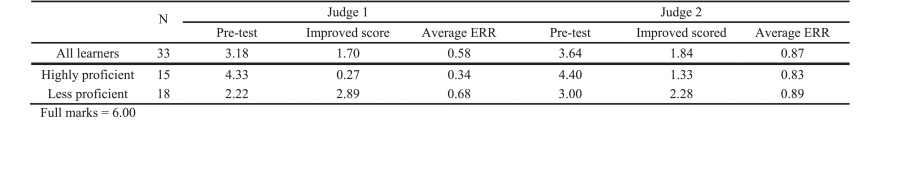
\includegraphics[width=15cm]{Table2.png}
%\counterwithin{figure}{section}
\centering
\caption{\textbf{Table II.} Data Frame-Payload}
\end{figure}

\paragraph{}
The data is framed in to a lightweight format[28] compatible with MQTT server. This
framed data is attached with the user, house and device details
as shown in Table II. To implement remote controlling of
devices through client application, the microcontroller reports
the status of the device whenever the state of device is
changed. To enable the billing utility process, the
microcontroller transmits the total power consumption of the
device every day to the servers via the MQTT protocol. Fig. 3
shows the prototype that was built in the lab to mimic the
proposed system.
\begin{figure}[H]
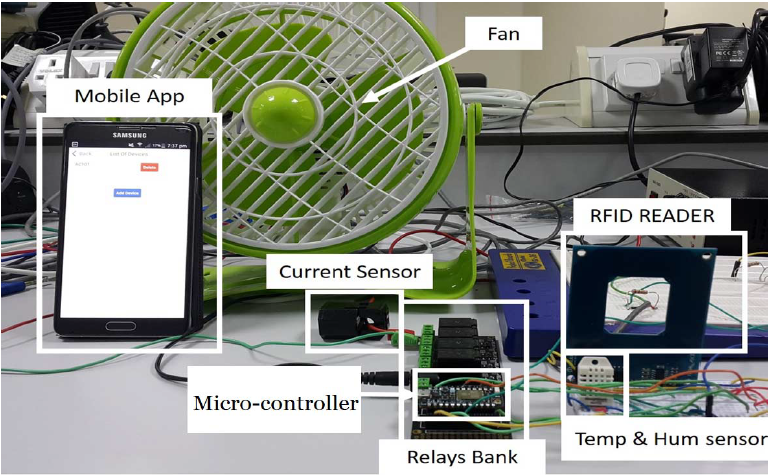
\includegraphics[height=8cm,width=16cm]{Figure3.png}
%\counterwithin{figure}{section}
\centering
\caption{\textbf{Figure 3.} Hardware Components}
\end{figure}

\subsection{Software}
\paragraph{}
The software implementation involves benchmarking and
data analysis techniques using Business Intelligence tool to
generate graphs, charts and reports in real time. This was
followed with the development of a mobile application to
render the generated graphs, charts, and reports to end users. A
description of these software modules is given as follows:

\begin{itemize}
    \item \textbf{Benchmarking and data analysis using BI platform}
    \newline
    One of the primary analysis techniques in data mining is
    benchmarking. Benchmarking the data sets can help identify which houses or residential areas should be focused on for
    setting optimal energy management goals and policies. The
    business intelligence software tool serves as an optimum
    platform for benchmarking real time data and generating userinteractive
    charts and reports. Different benchmarking
    scenarios are deemed for the four stakeholder levels as
    mentioned in the previous section. 
    \newpage
    For the stakeholder like a \textbf{home owner} in a residential area, they are entitled to view the
    graphs and charts for the total power consumption of his/her
    house on a daily, monthly, and annual basis. The user is
    prompted to enter his/her house ID and select the year for
    which he/she desires to view the power consumption of each
    device in the house as shown in Fig. 4. The home owners can
    use benchmarking service to compare their power
    consumption with other housing units that have a similar
    setup.
    \newline
        \begin{figure}[H]
        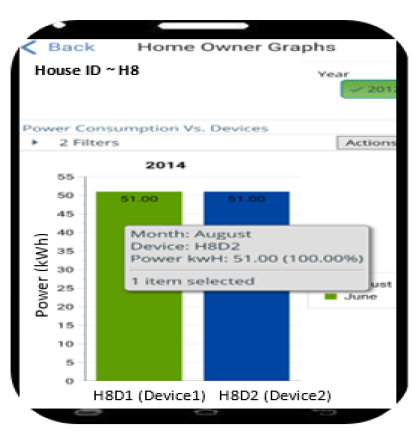
\includegraphics{Figure4.png}
        %\counterwithin{figure}{section}
        \centering
        \caption{\textbf{Figure 4.} Home Owner Graph}
        \end{figure}
    \newpage
    For \textbf{community stakeholders}, they are entitled to
    monitor power consumption of all houses in their respective
    community. There are two types of settings involved; first,
    benchmarking annual power consumption of each house
    against per square feet power consumption. Second,
    categorizing each house depending on its annual power
    consumption with respect to the house-age. The community
    owner is prompted to enter his/her respective community ID in
    order to obtain the desired graph or chart. A screenshot of
    annual power consumption chart for several housing units
    with their respective house IDs in a community is shown in
    Fig. 5.
    \newline
        \begin{figure}[H]
        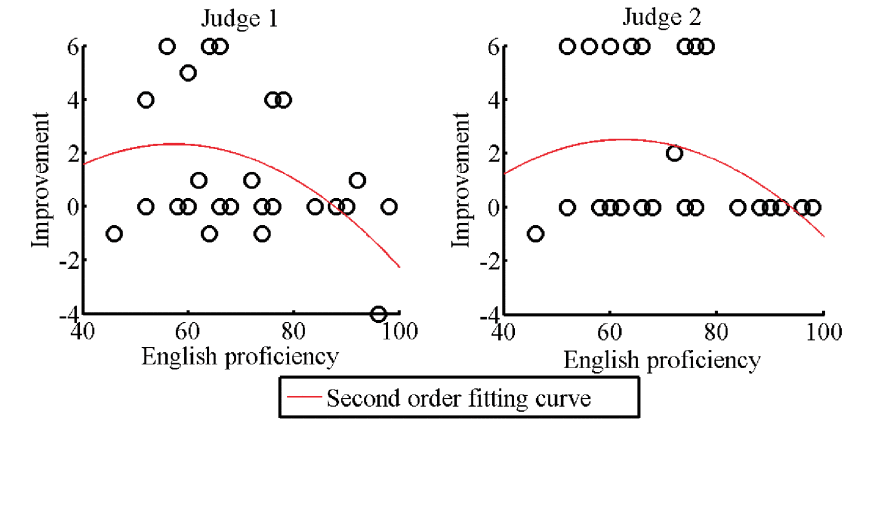
\includegraphics{Figure5.png}
        %\counterwithin{figure}{section}
        \centering
        \caption{\textbf{Figure 5.} Community Owner Graph}
        \end{figure}
    \newpage
    The \textbf{state stakeholders} at a state utility center can view data set distribution across
    regional communities within the state. Also, they can view the
    average power consumption spread across different
    communities on a monthly and yearly basis. The graphical
    data will be used to create benchmarks based on past records
    for conducting root cause analysis which is one of the business
    processes as mentioned previously. The trend line graphs can
    help predict the nature of power consumption of the state with
    respect to weather conditions (temperature) in future as shown
    in Fig.6.
    \newline
        \begin{figure}[H]
        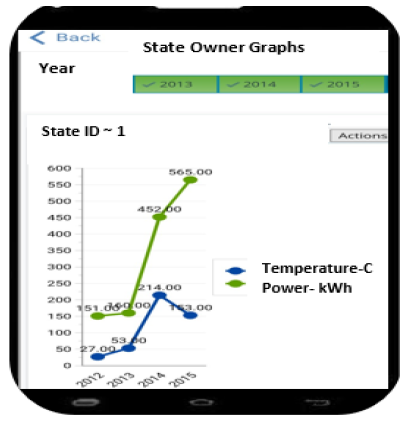
\includegraphics{Figure6.png}
        %\counterwithin{figure}{section}
        \centering
        \caption{\textbf{Figure 6.} State Owner Graph}
        \end{figure}
    \newpage
\item \textbf{Client Application}
        \newline
    A cross-platform application is developed which provides access
    to every stakeholder a different view to the data analytics
    according to his/her privileges. Once a user logs in, a service
    will run to get the user privileges and the user interface
    components that he/she will be able to see consequently.
    \newline For example, for the home owner, there are two services available:
    \newline First is monitoring power consumption data of each house device as shown in Fig. 6 and second is remote control
    services (ON/OFF) for house devices as shown in Fig. 7(a).
    For the bill tracking service, the user can view the monthly bill
    and pay the due amount online as shown in Fig. 7(b).
        \begin{figure}[H]
        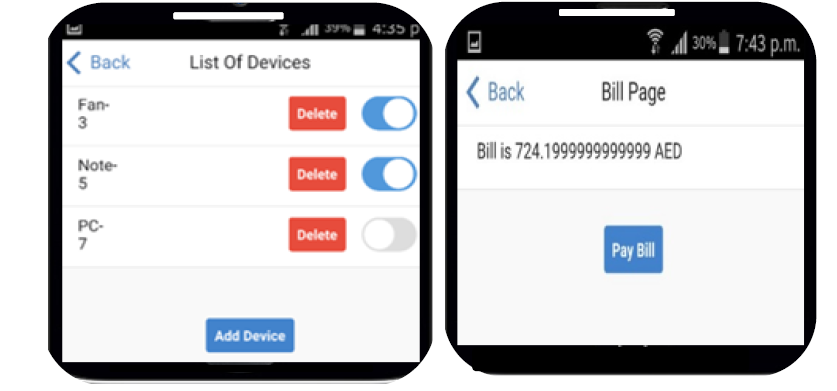
\includegraphics{Figure7.png}
        %\counterwithin{figure}{section}
        \centering
        \caption{\textbf{Figure 7.} (a) Remote control of devices \hspace{2ex} (b) Monthly Bill Management}
        \end{figure}
\end{itemize}

\newpage
\section{EVALUATION AND TESTING}
A set of criteria were developed to evaluate system
performance for scalability, speed and security. Scalability is
the main concern for the MQTT Server and Web server to
accommodate all customers on national level. Speed was also
important for querying to and from the storage server or
operational database. It’s worth mentioning that the security
aspect of the proposed system is under development.

\subsection{MQTT Server Scalability}
\paragraph{}
A network analysis tool was used to measure the following
metric: Throughput, Latency, and Packets dropped. For
an experimental comparison, a logarithmic scale of clients was
chosen to send 1, 10, 100, and 1000 consecutive messages
with a reliability of Quality of Service: QoS-0 and QoS-1 in
each case. QoS-2 was excluded in test cases due to its large
overhead. Table III represents different test case scenarios
indicating that the system was able to accept 1000 concurrent
MQTT clients publishing messages to a subscribed topic of
the MQTT server. 
\newline
    \begin{figure}[H]
    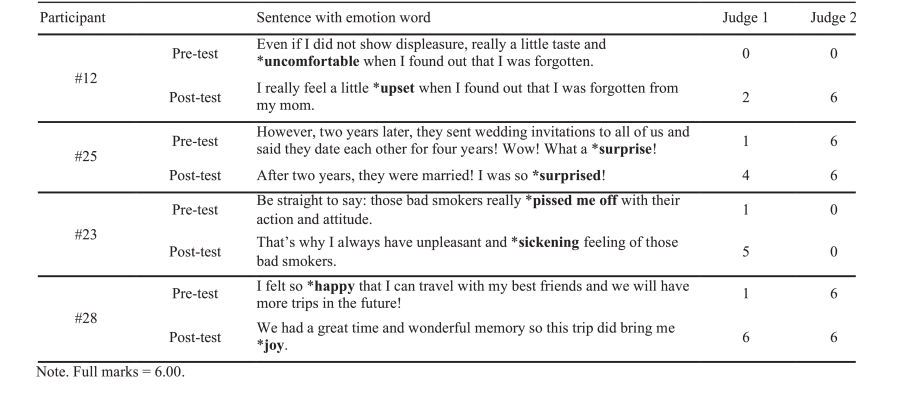
\includegraphics{Table3.png}
    %\counterwithin{figure}{section}
    \centering
    \caption{\textbf{Table III.} MQTT Test Cases and Results}
    \end{figure}
\newpage
From the results as shown in Table III, it is
evident that the overall latency for QoS-0 is always lower than
that for QoS-1 irrespective of the number of concurrent client
requests. This difference is expected because in
QoS-0 message delivery is not acknowledged whereas in QoS-
1 acknowledgment for confirmed message reception is sent,
which adds to the latency of message transmission in QoS-1.
Also, the throughput for QoS-1 was observed to be higher than
that for QoS-0 for any number of clients since QoS-1 offers a
reliable means of communication due to message
acknowledgement and persistent session (Fig. 8).
    \begin{figure}[H]
    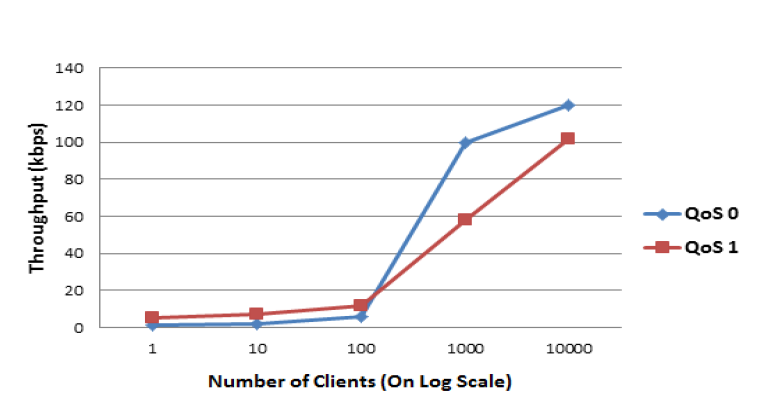
\includegraphics{Figure8.png}
    %\counterwithin{figure}{section}
    \centering
    \caption{\textbf{Figure 8.} Throughput (kbps) Vs. Number of clients’ graph}
    \end{figure}

\newpage
\subsection{Scalability for Webserver}
\paragraph{}
Many users were simulated concurrently using a Webserver
Stress Tool. Each user in this test makes a request involving
operational database. CPU and Network utilization were high
when all requests started coming as shown in Fig. 9. Almost
all requests were answered immediately up to 4000 users.
Beyond 4000 users the communication was terminated due to
data traffic congestion and testing tool limitation. Memory
remained about 85% throughout the test. This is due to
database read and writes activity that runs asynchronously in
the background.
    \begin{figure}[H]
    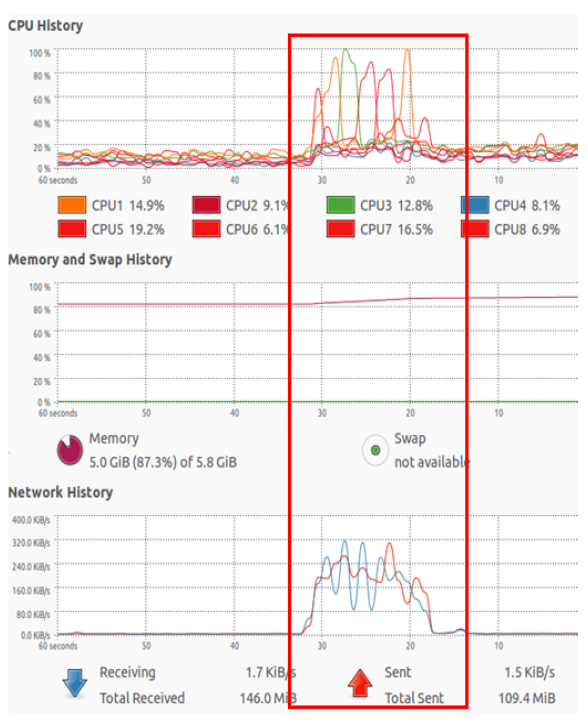
\includegraphics{Figure9.png}
    %\counterwithin{figure}{section}
    \centering
    \caption{\textbf{Figure 9.} Server performance during request phase}
    \end{figure}

\newpage
\subsection{Speed for Storage Server}
\paragraph{}
The data server speed was acceptable up to 4000 concurrent
users. This is again due to the data traffic congestion and
testing tool limitation. The time lapse for querying up to 4000
concurrent requests involved storage server operations. Read
operation was performed by the storage server using web
services. Moreover, an ETL (Extract-Transform-Load) script
was written to measure the time taken to read from storage
server during peak time. 4000 files, each 62 Bytes in size,
were extracted from the storage server for read operation. A
summary of the response time to complete read and write
operation by the storage server is shown in Table IV.
    \begin{figure}[H]
    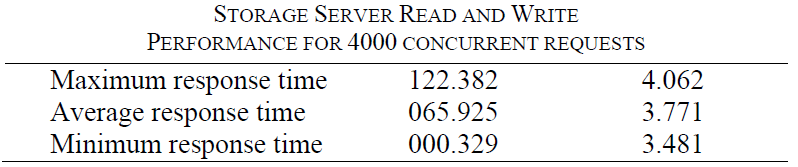
\includegraphics{Table4.png}
    %\counterwithin{figure}{section}
    \centering
    \caption{\textbf{Table IV.} Storage Server Performance}
    \end{figure}

\newpage
\section{CONCLUSION}
\paragraph{}
The proposed work is set to open new avenues for smart
energy management on IoT and Big Data platform. The
system design uses data analytics and scalable storage for
building a smart EMS to aid different stakeholders with their
respective privileges. The system empowers users to remotely
monitor and control devices, and online bill generation via a
friendly user interface mobile application

\newpage
% \cleardoublepage
% \addcontentsline{toc}{section}{\textbf{References}}
% \addcontentsline{}{section}{\textbf{References}}

\section{REFERENCES}
\begin{thebibliography}{9}

\bibitem{d}"A.R. Al-Ali, I.A. Zualkernan, M. Rashid, R. Gupta, M. Alikarar, "A smart home energy management system using IoT and big data analytics approach",\emph{IEEE Transactions on Consumer Electronics}, vol. 63, no. 4, pp. 426-434, 2017"
\bibitem{d}“Design and implementation of building energy monitoring and
management system based on wireless sensor networks,” \emph{Tenth International Conference on Computer Engineering \& Systems (ICCES)},
Cairo, 2015, pp. 230-233
\bibitem{d}N. H. Nguyen, Q. T. Tran, J. M. Leger and T. P. Vuong, “A real-time
control using wireless sensor network for intelligent energy management
system in buildings,” \emph{ 2010 IEEE Workshop on Environmental Energy
and Structural Monitoring Systems, Taranto}, 2010, pp. 87-92.
\bibitem{d}J. Byun, I. Hong, B. Kang and S. Park, “Implementation of an Adaptive
Intelligent Home Energy Management System Using a Wireless Ad-Hoc
and Sensor Network in Pervasive Environments,” \emph{Proceedings of
20th International Conference on Computer Communications and
Networks (ICCCN)}, Maui, HI, 2011, pp. 1-6.
\bibitem{d}J. Han, C. s. Choi, W. k. Park, I. Lee and S. h. Kim, “Smart home energy
management system including renewable energy based on ZigBee and PLC,”
\emph{IEEE Trans. Consumer Electron}, vol. 60, no. 2, pp. 198-202, May 2014.
\bibitem{d}J. Wang, J. Huang, W. Chen, J. Liu and D. Xu, “Design of IoT-based
energy efficiency management system for building ceramics production
line,” \emph{ IEEE 11th Conference on Industrial Electronics and
Applications (ICIEA)}, Hefei, 2016, pp. 912-917
\bibitem{d}G. Mingming, S. Liangshan, H. Xiaowei and S. Qingwei, “The System
of Wireless Smart House Based on GSM and ZigBee,” \emph{
International Conference on Intelligent Computation Technology and
Automation}, Changsha, 2010, pp. 1017-1020.
\bibitem{d}Serra, J., Pubill, D., Antonopoulos, A  and Verikoukis, C. “Smart HVAC constraints”, \emph{The Scientific World Journal}, 2014, pp 1-11.
\bibitem{d}Fong, K. F., Hanby, V. I., and Chow, T. T. “HVAC system optimization
for energy management by evolutionary programming,” Energy and
Buildings, 38(3), 2006, 220-231.
\bibitem{d}Tacklim Lee, Seonki Jeon, Dongjun Kang, Lee Won Park and Sehyun
Park, “Design and implementation of intelligent HVAC system based on
IoT and Bigdata platform,” \emph{IEEE International Conference on
Consumer Electronics (ICCE)}, Las Vegas, NV, 2017, pp. 398-399.
\bibitem{d}Y. T. Lee, W. H. Hsiao, C. M. Huang and S. C. T. Chou, “An integrated
cloud-based smart home management system with community
hierarchy,” \emph{IEEE Trans. Consumer Electron}, vol. 62, no. 1, pp. 1-9, Feb.
2016.
\bibitem{d}E. Rodriguez-Diaz, J. C. Vasquez and J. M. Guerrero, “Intelligent DC
Homes in Future Sustainable Energy Systems: When efficiency and
intelligence work together,” \emph{IEEE Consumer Electron. Magazine}, vol. 5,
no. 1, pp. 74-80, Jan. 2016.
\bibitem{d}D. S. Kim, S. Y. Son and J. Lee, “Developments of the in-home display
systems for residential energy monitoring,” \emph{IEEE Trans. Consumer
Electron}, vol. 59, no. 3, pp. 492-498, August 2013.
\bibitem{d}Y. S. Son, T. Pulkkinen, K. D. Moon and C. Kim, “Home energy
management system based on power line communication,” \emph{IEEE Trans.
Consumer Electron}, vol. 56, no. 3, pp. 1380-1386, Aug. 2010.
\bibitem{d}N. Kushiro, S. Suzuki, M. Nakata, H. Takahara and M. Inoue,
“Integrated residential gateway controller for home energy management
system,” in\emph{ IEEE Transactions on Consumer Electronics}, vol. 49, no. 3,
pp. 629-636, Aug. 2003.
\bibitem{d}M. Erol-Kantarci and H. T. Mouftah, “Wireless Sensor Networks for
Cost-Efficient Residential Energy Management in the Smart Grid,” in\emph{
IEEE Transactions on Smart Grid}, vol. 2, no. 2, pp. 314-325, June 2011.
\bibitem{d}T. Fiedler and P. M. Mircea, “Energy management systems according to
the ISO 50001 standard — Challenges and benefits,” \emph{ International
Conference on Applied and Theoretical Electricity (ICATE)}, Craiova,
2012, pp. 1-4.
\bibitem{d}K. Dittawit and F. A. Aagesen, “Home energy management system for
electricity cost savings and comfort preservation,” \emph{IEEE Fourth
International Conference on Consumer Electronics Berlin (ICCEBerlin),}
Berlin, 2014, pp. 309-313.

\end{thebibliography}
\end{document}